%
% API Documentation for Project
% Include File
%
% Generated by epydoc 3.0.1
% [Fri Dec  9 04:12:59 2016]
%
\documentclass[oneside]{book}
\usepackage{alltt, parskip, fancyhdr, boxedminipage}
\usepackage{makeidx, multirow, longtable, tocbibind, amssymb}
\usepackage{fullpage}
\usepackage[usenames]{color}
\usepackage[final]{pdfpages}
\usepackage{graphicx}
\usepackage{float}
\usepackage{listings}
\setlength{\headheight}{16pt}
\setlength{\headsep}{24pt}
\setlength{\topmargin}{-\headsep}
\setlength{\parindent}{0ex}
\setlength{\parskip}{2ex}
\setlength{\fboxrule}{2\fboxrule}
\newlength{\BCL} % base class length, for base trees.
\pagestyle{fancy}
\renewcommand{\sectionmark}[1]{\markboth{#1}{}}
\renewcommand{\subsectionmark}[1]{\markright{#1}}
\definecolor{py@keywordcolour}{rgb}{1,0.45882,0}
\definecolor{py@stringcolour}{rgb}{0,0.666666,0}
\definecolor{py@commentcolour}{rgb}{1,0,0}
\definecolor{py@ps1colour}{rgb}{0.60784,0,0}
\definecolor{py@ps2colour}{rgb}{0.60784,0,1}
\definecolor{py@inputcolour}{rgb}{0,0,0}
\definecolor{py@outputcolour}{rgb}{0,0,1}
\definecolor{py@exceptcolour}{rgb}{1,0,0}
\definecolor{py@defnamecolour}{rgb}{1,0.5,0.5}
\definecolor{py@builtincolour}{rgb}{0.58039,0,0.58039}
\definecolor{py@identifiercolour}{rgb}{0,0,0}
\definecolor{py@linenumcolour}{rgb}{0.4,0.4,0.4}
\definecolor{py@inputcolour}{rgb}{0,0,0}
% Prompt
\newcommand{\pysrcprompt}[1]{\textcolor{py@ps1colour}{\small\textbf{#1}}}
\newcommand{\pysrcmore}[1]{\textcolor{py@ps2colour}{\small\textbf{#1}}}
% Source code
\newcommand{\pysrckeyword}[1]{\textcolor{py@keywordcolour}{\small\textbf{#1}}}
\newcommand{\pysrcbuiltin}[1]{\textcolor{py@builtincolour}{\small\textbf{#1}}}
\newcommand{\pysrcstring}[1]{\textcolor{py@stringcolour}{\small\textbf{#1}}}
\newcommand{\pysrcdefname}[1]{\textcolor{py@defnamecolour}{\small\textbf{#1}}}
\newcommand{\pysrcother}[1]{\small\textbf{#1}}
% Comments
\newcommand{\pysrccomment}[1]{\textcolor{py@commentcolour}{\small\textbf{#1}}}
% Output
\newcommand{\pysrcoutput}[1]{\textcolor{py@outputcolour}{\small\textbf{#1}}}
% Exceptions
\newcommand{\pysrcexcept}[1]{\textcolor{py@exceptcolour}{\small\textbf{#1}}}
\newlength{\funcindent}
\newlength{\funcwidth}
\setlength{\funcindent}{1cm}
\setlength{\funcwidth}{\textwidth}
\addtolength{\funcwidth}{-2\funcindent}
\newlength{\varindent}
\newlength{\varnamewidth}
\newlength{\vardescrwidth}
\newlength{\varwidth}
\setlength{\varindent}{1cm}
\setlength{\varnamewidth}{.3\textwidth}
\setlength{\varwidth}{\textwidth}
\addtolength{\varwidth}{-4\tabcolsep}
\addtolength{\varwidth}{-3\arrayrulewidth}
\addtolength{\varwidth}{-2\varindent}
\setlength{\vardescrwidth}{\varwidth}
\addtolength{\vardescrwidth}{-\varnamewidth}
\newenvironment{Ventry}[1]%
 {\begin{list}{}{%
   \renewcommand{\makelabel}[1]{\texttt{##1:}\hfil}%
   \settowidth{\labelwidth}{\texttt{#1:}}%
   \setlength{\leftmargin}{\labelsep}%
   \addtolength{\leftmargin}{\labelwidth}}}%
 {\end{list}}
\usepackage[utf8]{inputenc}
\definecolor{UrlColor}{rgb}{0,0.08,0.45}
\usepackage[dvips, pagebackref, pdftitle={Project}, pdfcreator={epydoc 3.0.1}, bookmarks=true, bookmarksopen=false, pdfpagemode=UseOutlines, colorlinks=true, linkcolor=black, anchorcolor=black, citecolor=black, filecolor=black, menucolor=black, pagecolor=black, urlcolor=UrlColor]{hyperref}
\makeindex

\begin{document}

%%%%%%%%%%%%%%%%%%%%%%%%%%%%%%%%%%%%%%%%%%%%%%%%%%%%%%%%%%%%%%%%%%%%%%%%%%%
%%                                Header                                 %%
%%%%%%%%%%%%%%%%%%%%%%%%%%%%%%%%%%%%%%%%%%%%%%%%%%%%%%%%%%%%%%%%%%%%%%%%%%%


%%%%%%%%%%%%%%%%%%%%%%%%%%%%%%%%%%%%%%%%%%%%%%%%%%%%%%%%%%%%%%%%%%%%%%%%%%%
%%                                 Title                                 %%
%%%%%%%%%%%%%%%%%%%%%%%%%%%%%%%%%%%%%%%%%%%%%%%%%%%%%%%%%%%%%%%%%%%%%%%%%%%

\title {Detección de sexismo en Twitter \\ Ingeniería de Software}
\author{Abraham Solís Álvarez \\ Mario Alejandro Gil Lázaro}
\date{December 8, 2016}
\maketitle

%%%%%%%%%%%%%%%%%%%%%%%%%%%%%%%%%%%%%%%%%%%%%%%%%%%%%%%%%%%%%%%%%%%%%%%%%%%
%%                           Table of Contents                           %%
%%%%%%%%%%%%%%%%%%%%%%%%%%%%%%%%%%%%%%%%%%%%%%%%%%%%%%%%%%%%%%%%%%%%%%%%%%%

%\addtolength{\parskip}{-2ex}
\tableofcontents
%\addtolength{\parskip}{2ex}

%%%%%%%%%%%%%%%%%%%%%%%%%%%%%%%%%%%%%%%%%%%%%%%%%%%%%%%%%%%%%%%%%%%%%%%%%%%
%%                               Includes                                %%
%%%%%%%%%%%%%%%%%%%%%%%%%%%%%%%%%%%%%%%%%%%%%%%%%%%%%%%%%%%%%%%%%%%%%%%%%%%
\chapter{Requerimientos}
\section{Requerimientos}
\subsection{Descripción del proyecto}
Este proyecto busca determinar los niveles de sexismo y otras manifestaciones
de odio y discriminación, en el texto que los usuarios del sitio de
microblogeo Twitter, escriben diariamente. Dado que el internet es una
plataforma moderna de expresión y debido también a que la ya mencionada red
social posee un número importante de usuarios, consideramos que la información
ahí recabada representa una muestra importante. Así mismo, el hecho de que
los medios virtuales son comúnmente considerados como medios poco
trascendentales, en los que se puede supuestamente evitar las consecuencias
que los propios comentarios puedan ocasionar, creemos que las opiniones ahí
expresadas poseen un alto grado de sinceridad, mayor al que podría obtenerse
en el discurso hablado.

\subsection{Requerimientos del proyecto}
El sistema propuesto debe ser capaz de recolectar los posts directamente del
stream de Twitter, convertir los datos al formato que mejor convenga, etiquetar
palabra por palabra el texto, y realizar mediciones que permitan elaborar
indicadores que arrojen luz sobre las costumbres y la cultura de los usuarios
de la red social. Se pretende lograr esto manteniendo los más altos estándares
de calidad que sea posible, aplicando prácticas de programación modernas.

\subsection{Dependencias}
Para ejecutar el programa con las mayores probabilidades de éxito se recomienda
utilizar un sistema operativo basado en GNU/Linux. Es necesario instalar una
Python 3.x, de preferencia la versión 3.5, que fue la utilizada en el
desarrollo del sistema. Se recomienda utilizar el programa `pip` para instalar
los módulos de Python `nltk` y `plac`, que son necesarios para ejecutar el
programa. Es necesario contar con una conexión a internet.

\chapter{Desarrollo}
\section{Desarrollo}
\subsection{Cronograma de Actividades}
\begin{figure}[H]
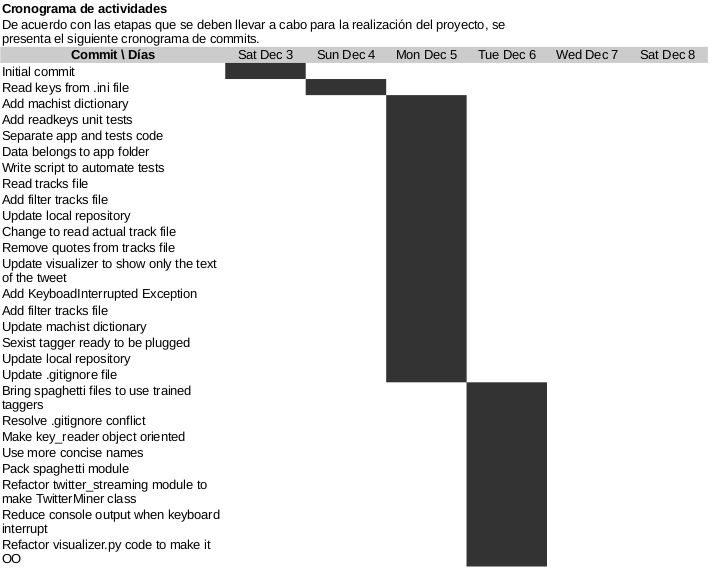
\includegraphics[scale=0.5]{crono1.png}
\end{figure}
\begin{figure}[H]
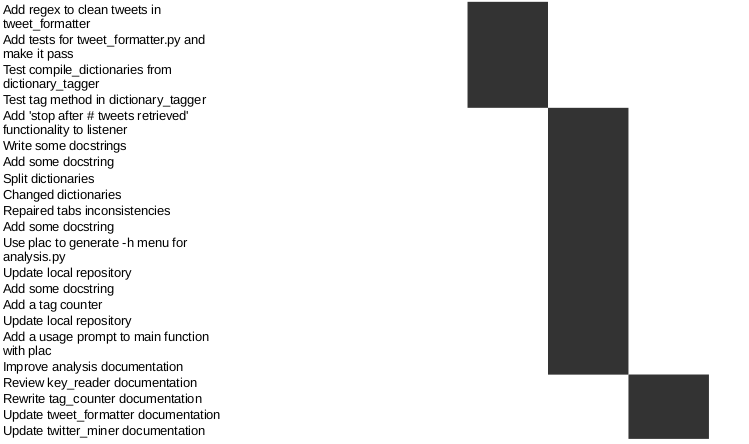
\includegraphics[scale=0.5]{crono2.png}
\end{figure}
\subsection{Reportes de Revisiones técnicas e informales}
La información de los reportes y bugs que se fueron corrigiendo aparecen en los commits hechos en la url del proyecto.
\url{https://github.com/azaroma/analisis-machismo}
\subsection{Bugs corregidos}
La información de los reportes y bugs que se fueron corrigiendo aparecen en los commits hechos en la url del proyecto.
\url{https://github.com/azaroma/analisis-machismo} 

\chapter{Documentación}
\section{Documentación}
\subsection{Cómo se usa el software}
Por el momento, la única forma de interactuar con el sistema es mediante el
módulo `analysis.py`, localizado en el directorio `app` (con el comando
`python analysis.py`). Tenga en cuenta que usted debe estar localizado dentro
de dicho directorio. Además, se proporciona un script que ejecuta las pruebas
del sistema en el directorio raíz: `run\_tests`.

\subsection{Documentación de las funciones internas}
\begin{figure}[H]
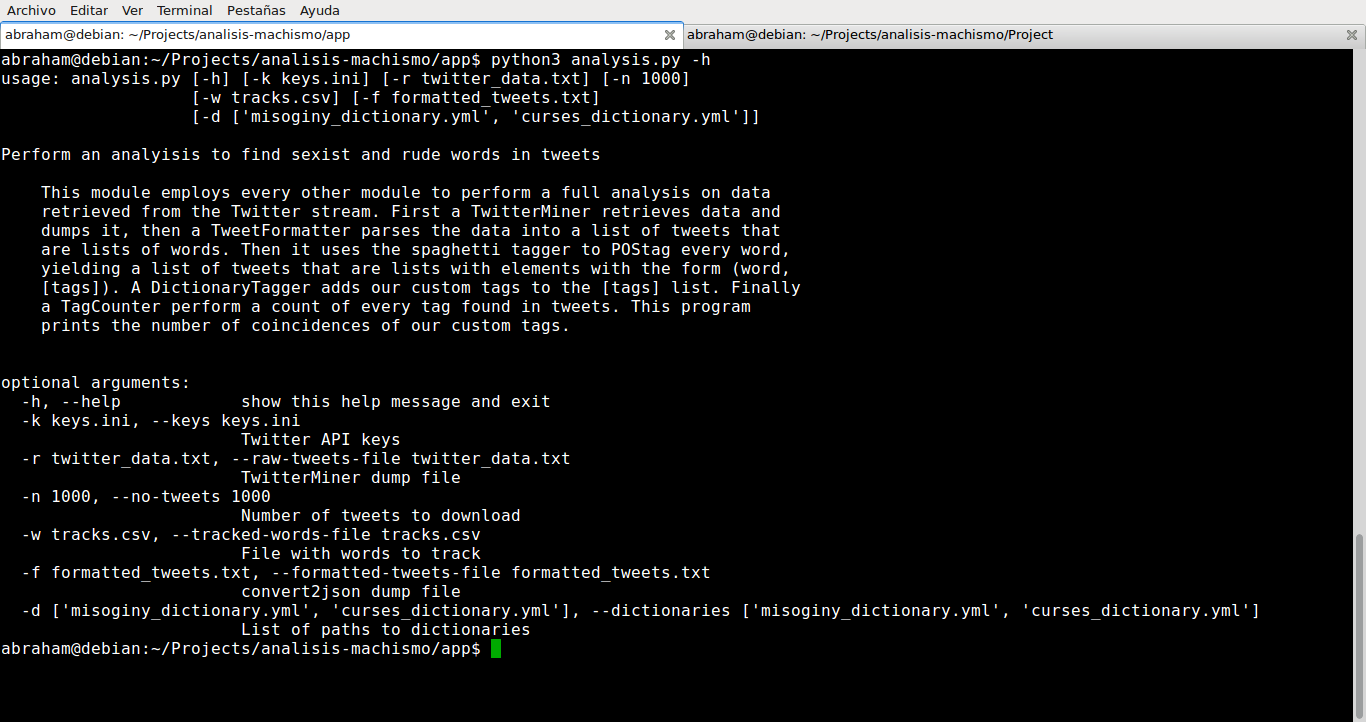
\includegraphics[scale=0.35]{help.png}
\end{figure}

%
% API Documentation for Project
% Package analisis-machismo
%
% Generated by epydoc 3.0.1
% [Thu Dec  8 01:51:18 2016]
%

%%%%%%%%%%%%%%%%%%%%%%%%%%%%%%%%%%%%%%%%%%%%%%%%%%%%%%%%%%%%%%%%%%%%%%%%%%%
%%                          Module Description                           %%
%%%%%%%%%%%%%%%%%%%%%%%%%%%%%%%%%%%%%%%%%%%%%%%%%%%%%%%%%%%%%%%%%%%%%%%%%%%

    \index{analisis-machismo \textit{(package)}|(}
\section{Package analisis-machismo}

    \label{analisis-machismo}
    \index{analisis-machismo \textit{(package)}|)}

%
% API Documentation for Project
% Package analisis-machismo.app
%
% Generated by epydoc 3.0.1
% [Fri Dec  9 04:12:59 2016]
%

%%%%%%%%%%%%%%%%%%%%%%%%%%%%%%%%%%%%%%%%%%%%%%%%%%%%%%%%%%%%%%%%%%%%%%%%%%%
%%                          Module Description                           %%
%%%%%%%%%%%%%%%%%%%%%%%%%%%%%%%%%%%%%%%%%%%%%%%%%%%%%%%%%%%%%%%%%%%%%%%%%%%

    \index{analisis-machismo \textit{(package)}!analisis-machismo.app \textit{(package)}|(}
\section{Package analisis-machismo.app}

    \label{analisis-machismo:app}

%%%%%%%%%%%%%%%%%%%%%%%%%%%%%%%%%%%%%%%%%%%%%%%%%%%%%%%%%%%%%%%%%%%%%%%%%%%
%%                                Modules                                %%
%%%%%%%%%%%%%%%%%%%%%%%%%%%%%%%%%%%%%%%%%%%%%%%%%%%%%%%%%%%%%%%%%%%%%%%%%%%

\subsection{Modules}

\begin{itemize}
\setlength{\parskip}{0ex}
\item \textbf{analysis}
  \textit{(Section \ref{analisis-machismo:app:analysis}, p.~\pageref{analisis-machismo:app:analysis})}

\item \textbf{dictionary\_tagger}
  \textit{(Section \ref{analisis-machismo:app:dictionary_tagger}, p.~\pageref{analisis-machismo:app:dictionary_tagger})}

\item \textbf{key\_reader}
  \textit{(Section \ref{analisis-machismo:app:key_reader}, p.~\pageref{analisis-machismo:app:key_reader})}

\item \textbf{tag\_counter}
  \textit{(Section \ref{analisis-machismo:app:tag_counter}, p.~\pageref{analisis-machismo:app:tag_counter})}

\item \textbf{tweet\_formatter}
  \textit{(Section \ref{analisis-machismo:app:tweet_formatter}, p.~\pageref{analisis-machismo:app:tweet_formatter})}

\item \textbf{twitter\_miner}
  \textit{(Section \ref{analisis-machismo:app:twitter_miner}, p.~\pageref{analisis-machismo:app:twitter_miner})}

\end{itemize}

    \index{analisis-machismo \textit{(package)}!analisis-machismo.app \textit{(package)}|)}

%
% API Documentation for Project
% Module analisis-machismo.app.analysis
%
% Generated by epydoc 3.0.1
% [Fri Dec  9 04:12:59 2016]
%

%%%%%%%%%%%%%%%%%%%%%%%%%%%%%%%%%%%%%%%%%%%%%%%%%%%%%%%%%%%%%%%%%%%%%%%%%%%
%%                          Module Description                           %%
%%%%%%%%%%%%%%%%%%%%%%%%%%%%%%%%%%%%%%%%%%%%%%%%%%%%%%%%%%%%%%%%%%%%%%%%%%%

    \index{analisis-machismo \textit{(package)}!analisis-machismo.app \textit{(package)}!analisis-machismo.app.analysis \textit{(module)}|(}
\section{Module analisis-machismo.app.analysis}

    \label{analisis-machismo:app:analysis}

%%%%%%%%%%%%%%%%%%%%%%%%%%%%%%%%%%%%%%%%%%%%%%%%%%%%%%%%%%%%%%%%%%%%%%%%%%%
%%                               Functions                               %%
%%%%%%%%%%%%%%%%%%%%%%%%%%%%%%%%%%%%%%%%%%%%%%%%%%%%%%%%%%%%%%%%%%%%%%%%%%%

  \subsection{Functions}

    \label{analisis-machismo:app:analysis:main}
    \index{analisis-machismo \textit{(package)}!analisis-machismo.app \textit{(package)}!analisis-machismo.app.analysis \textit{(module)}!analisis-machismo.app.analysis.main \textit{(function)}}

    \vspace{0.5ex}

\hspace{.8\funcindent}\begin{boxedminipage}{\funcwidth}

    \raggedright \textbf{main}(\textit{keys}={\tt 'keys.ini'}, \textit{raw\_tweets\_file}={\tt 'twitter\_data.txt'}, \textit{no\_tweets}={\tt 1000}, \textit{tracked\_words\_file}={\tt 'tracks.csv'}, \textit{formatted\_tweets\_file}={\tt 'formatted\_tweets.txt'}, \textit{dictionaries}={\tt ['misoginy\_dictionary.yml','curses\_dictionary.yml']})

    \vspace{-1.5ex}

    \rule{\textwidth}{0.5\fboxrule}
\setlength{\parskip}{2ex}
    Perform an analyisis to find sexist and rude words in tweets

    This module employs every other module to perform a full analysis on 
    data retrieved from the Twitter stream. First a TwitterMiner retrieves 
    data and dumps it, then a TweetFormatter parses the data into a list of
    tweets that are lists of words. Then it uses the spaghetti tagger to 
    POStag every word, yielding a list of tweets that are lists with 
    elements with the form (word, [tags]). A DictionaryTagger adds our 
    custom tags to the [tags] list. Finally a TagCounter perform a count of
    every tag found in tweets. This program prints the number of 
    coincidences of our custom tags.

\setlength{\parskip}{1ex}
    \end{boxedminipage}

    \index{analisis-machismo \textit{(package)}!analisis-machismo.app \textit{(package)}!analisis-machismo.app.analysis \textit{(module)}|)}

%
% API Documentation for Project
% Module analisis-machismo.app.dictionary_tagger
%
% Generated by epydoc 3.0.1
% [Fri Dec  9 04:12:59 2016]
%

%%%%%%%%%%%%%%%%%%%%%%%%%%%%%%%%%%%%%%%%%%%%%%%%%%%%%%%%%%%%%%%%%%%%%%%%%%%
%%                          Module Description                           %%
%%%%%%%%%%%%%%%%%%%%%%%%%%%%%%%%%%%%%%%%%%%%%%%%%%%%%%%%%%%%%%%%%%%%%%%%%%%

    \index{analisis-machismo \textit{(package)}!analisis-machismo.app \textit{(package)}!analisis-machismo.app.dictionary\_tagger \textit{(module)}|(}
\section{Module analisis-machismo.app.dictionary\_tagger}

    \label{analisis-machismo:app:dictionary_tagger}

%%%%%%%%%%%%%%%%%%%%%%%%%%%%%%%%%%%%%%%%%%%%%%%%%%%%%%%%%%%%%%%%%%%%%%%%%%%
%%                           Class Description                           %%
%%%%%%%%%%%%%%%%%%%%%%%%%%%%%%%%%%%%%%%%%%%%%%%%%%%%%%%%%%%%%%%%%%%%%%%%%%%

    \index{analisis-machismo \textit{(package)}!analisis-machismo.app \textit{(package)}!analisis-machismo.app.dictionary\_tagger \textit{(module)}!analisis-machismo.app.dictionary\_tagger.DictionaryTagger \textit{(class)}|(}
\subsection{Class DictionaryTagger}

    \label{analisis-machismo:app:dictionary_tagger:DictionaryTagger}
Python class for tagging text with dictionaries


%%%%%%%%%%%%%%%%%%%%%%%%%%%%%%%%%%%%%%%%%%%%%%%%%%%%%%%%%%%%%%%%%%%%%%%%%%%
%%                                Methods                                %%
%%%%%%%%%%%%%%%%%%%%%%%%%%%%%%%%%%%%%%%%%%%%%%%%%%%%%%%%%%%%%%%%%%%%%%%%%%%

  \subsubsection{Methods}

    \label{analisis-machismo:app:dictionary_tagger:DictionaryTagger:__init__}
    \index{analisis-machismo \textit{(package)}!analisis-machismo.app \textit{(package)}!analisis-machismo.app.dictionary\_tagger \textit{(module)}!analisis-machismo.app.dictionary\_tagger.DictionaryTagger \textit{(class)}!analisis-machismo.app.dictionary\_tagger.DictionaryTagger.\_\_init\_\_ \textit{(method)}}

    \vspace{0.5ex}

\hspace{.8\funcindent}\begin{boxedminipage}{\funcwidth}

    \raggedright \textbf{\_\_init\_\_}(\textit{self}, \textit{dictionary\_paths})

    \vspace{-1.5ex}

    \rule{\textwidth}{0.5\fboxrule}
\setlength{\parskip}{2ex}
    Dictionary is a dict containing all the dictionaries parsed from the 
    paths given.

\setlength{\parskip}{1ex}
    \end{boxedminipage}

    \label{analisis-machismo:app:dictionary_tagger:DictionaryTagger:compile_dictionaries}
    \index{analisis-machismo \textit{(package)}!analisis-machismo.app \textit{(package)}!analisis-machismo.app.dictionary\_tagger \textit{(module)}!analisis-machismo.app.dictionary\_tagger.DictionaryTagger \textit{(class)}!analisis-machismo.app.dictionary\_tagger.DictionaryTagger.compile\_dictionaries \textit{(method)}}

    \vspace{0.5ex}

\hspace{.8\funcindent}\begin{boxedminipage}{\funcwidth}

    \raggedright \textbf{compile\_dictionaries}(\textit{self}, \textit{dictionary\_paths})

    \vspace{-1.5ex}

    \rule{\textwidth}{0.5\fboxrule}
\setlength{\parskip}{2ex}
    Returns a list of dictionaries parsed from .yml files

\setlength{\parskip}{1ex}
    \end{boxedminipage}

    \label{analisis-machismo:app:dictionary_tagger:DictionaryTagger:tag}
    \index{analisis-machismo \textit{(package)}!analisis-machismo.app \textit{(package)}!analisis-machismo.app.dictionary\_tagger \textit{(module)}!analisis-machismo.app.dictionary\_tagger.DictionaryTagger \textit{(class)}!analisis-machismo.app.dictionary\_tagger.DictionaryTagger.tag \textit{(method)}}

    \vspace{0.5ex}

\hspace{.8\funcindent}\begin{boxedminipage}{\funcwidth}

    \raggedright \textbf{tag}(\textit{self}, \textit{postagged\_sentences})

\setlength{\parskip}{2ex}
\setlength{\parskip}{1ex}
    \end{boxedminipage}

    \label{analisis-machismo:app:dictionary_tagger:DictionaryTagger:tag_sentence}
    \index{analisis-machismo \textit{(package)}!analisis-machismo.app \textit{(package)}!analisis-machismo.app.dictionary\_tagger \textit{(module)}!analisis-machismo.app.dictionary\_tagger.DictionaryTagger \textit{(class)}!analisis-machismo.app.dictionary\_tagger.DictionaryTagger.tag\_sentence \textit{(method)}}

    \vspace{0.5ex}

\hspace{.8\funcindent}\begin{boxedminipage}{\funcwidth}

    \raggedright \textbf{tag\_sentence}(\textit{self}, \textit{sentence}, \textit{tag\_with\_lemmas}={\tt None})

    \vspace{-1.5ex}

    \rule{\textwidth}{0.5\fboxrule}
\setlength{\parskip}{2ex}
    The result is only tagging of all the possible ones. The resulting 
    taging is determined by these two priority rules:

    \begin{itemize}
    \setlength{\parskip}{0.6ex}
      \item longest matches have higher priority

      \item search is made left to right

    \end{itemize}

\setlength{\parskip}{1ex}
    \end{boxedminipage}

    \index{analisis-machismo \textit{(package)}!analisis-machismo.app \textit{(package)}!analisis-machismo.app.dictionary\_tagger \textit{(module)}!analisis-machismo.app.dictionary\_tagger.DictionaryTagger \textit{(class)}|)}
    \index{analisis-machismo \textit{(package)}!analisis-machismo.app \textit{(package)}!analisis-machismo.app.dictionary\_tagger \textit{(module)}|)}

%
% API Documentation for Project
% Module analisis-machismo.app.key_reader
%
% Generated by epydoc 3.0.1
% [Fri Dec  9 04:12:59 2016]
%

%%%%%%%%%%%%%%%%%%%%%%%%%%%%%%%%%%%%%%%%%%%%%%%%%%%%%%%%%%%%%%%%%%%%%%%%%%%
%%                          Module Description                           %%
%%%%%%%%%%%%%%%%%%%%%%%%%%%%%%%%%%%%%%%%%%%%%%%%%%%%%%%%%%%%%%%%%%%%%%%%%%%

    \index{analisis-machismo \textit{(package)}!analisis-machismo.app \textit{(package)}!analisis-machismo.app.key\_reader \textit{(module)}|(}
\section{Module analisis-machismo.app.key\_reader}

    \label{analisis-machismo:app:key_reader}

%%%%%%%%%%%%%%%%%%%%%%%%%%%%%%%%%%%%%%%%%%%%%%%%%%%%%%%%%%%%%%%%%%%%%%%%%%%
%%                           Class Description                           %%
%%%%%%%%%%%%%%%%%%%%%%%%%%%%%%%%%%%%%%%%%%%%%%%%%%%%%%%%%%%%%%%%%%%%%%%%%%%

    \index{analisis-machismo \textit{(package)}!analisis-machismo.app \textit{(package)}!analisis-machismo.app.key\_reader \textit{(module)}!analisis-machismo.app.key\_reader.KeyReader \textit{(class)}|(}
\subsection{Class KeyReader}

    \label{analisis-machismo:app:key_reader:KeyReader}
Wrapper of ConfigParser to load .ini file with Twitter API keys


%%%%%%%%%%%%%%%%%%%%%%%%%%%%%%%%%%%%%%%%%%%%%%%%%%%%%%%%%%%%%%%%%%%%%%%%%%%
%%                                Methods                                %%
%%%%%%%%%%%%%%%%%%%%%%%%%%%%%%%%%%%%%%%%%%%%%%%%%%%%%%%%%%%%%%%%%%%%%%%%%%%

  \subsubsection{Methods}

    \label{analisis-machismo:app:key_reader:KeyReader:__init__}
    \index{analisis-machismo \textit{(package)}!analisis-machismo.app \textit{(package)}!analisis-machismo.app.key\_reader \textit{(module)}!analisis-machismo.app.key\_reader.KeyReader \textit{(class)}!analisis-machismo.app.key\_reader.KeyReader.\_\_init\_\_ \textit{(method)}}

    \vspace{0.5ex}

\hspace{.8\funcindent}\begin{boxedminipage}{\funcwidth}

    \raggedright \textbf{\_\_init\_\_}(\textit{self})

\setlength{\parskip}{2ex}
\setlength{\parskip}{1ex}
    \end{boxedminipage}

    \label{analisis-machismo:app:key_reader:KeyReader:read}
    \index{analisis-machismo \textit{(package)}!analisis-machismo.app \textit{(package)}!analisis-machismo.app.key\_reader \textit{(module)}!analisis-machismo.app.key\_reader.KeyReader \textit{(class)}!analisis-machismo.app.key\_reader.KeyReader.read \textit{(method)}}

    \vspace{0.5ex}

\hspace{.8\funcindent}\begin{boxedminipage}{\funcwidth}

    \raggedright \textbf{read}(\textit{self}, \textit{filename}={\tt 'keys.ini'}, \textit{section}={\tt 'keys'})

    \vspace{-1.5ex}

    \rule{\textwidth}{0.5\fboxrule}
\setlength{\parskip}{2ex}
    Import the configparser, tell it to read the file, and get a listing of
    the sections. Sections are listed in a python dictionary.

\setlength{\parskip}{1ex}
    \end{boxedminipage}

    \index{analisis-machismo \textit{(package)}!analisis-machismo.app \textit{(package)}!analisis-machismo.app.key\_reader \textit{(module)}!analisis-machismo.app.key\_reader.KeyReader \textit{(class)}|)}
    \index{analisis-machismo \textit{(package)}!analisis-machismo.app \textit{(package)}!analisis-machismo.app.key\_reader \textit{(module)}|)}

%
% API Documentation for Project
% Module analisis-machismo.app.tag_counter
%
% Generated by epydoc 3.0.1
% [Fri Dec  9 04:13:00 2016]
%

%%%%%%%%%%%%%%%%%%%%%%%%%%%%%%%%%%%%%%%%%%%%%%%%%%%%%%%%%%%%%%%%%%%%%%%%%%%
%%                          Module Description                           %%
%%%%%%%%%%%%%%%%%%%%%%%%%%%%%%%%%%%%%%%%%%%%%%%%%%%%%%%%%%%%%%%%%%%%%%%%%%%

    \index{analisis-machismo \textit{(package)}!analisis-machismo.app \textit{(package)}!analisis-machismo.app.tag\_counter \textit{(module)}|(}
\section{Module analisis-machismo.app.tag\_counter}

    \label{analisis-machismo:app:tag_counter}

%%%%%%%%%%%%%%%%%%%%%%%%%%%%%%%%%%%%%%%%%%%%%%%%%%%%%%%%%%%%%%%%%%%%%%%%%%%
%%                           Class Description                           %%
%%%%%%%%%%%%%%%%%%%%%%%%%%%%%%%%%%%%%%%%%%%%%%%%%%%%%%%%%%%%%%%%%%%%%%%%%%%

    \index{analisis-machismo \textit{(package)}!analisis-machismo.app \textit{(package)}!analisis-machismo.app.tag\_counter \textit{(module)}!analisis-machismo.app.tag\_counter.TagCounter \textit{(class)}|(}
\subsection{Class TagCounter}

    \label{analisis-machismo:app:tag_counter:TagCounter}
Wrapper for a tag counting method


%%%%%%%%%%%%%%%%%%%%%%%%%%%%%%%%%%%%%%%%%%%%%%%%%%%%%%%%%%%%%%%%%%%%%%%%%%%
%%                                Methods                                %%
%%%%%%%%%%%%%%%%%%%%%%%%%%%%%%%%%%%%%%%%%%%%%%%%%%%%%%%%%%%%%%%%%%%%%%%%%%%

  \subsubsection{Methods}

    \label{analisis-machismo:app:tag_counter:TagCounter:__init__}
    \index{analisis-machismo \textit{(package)}!analisis-machismo.app \textit{(package)}!analisis-machismo.app.tag\_counter \textit{(module)}!analisis-machismo.app.tag\_counter.TagCounter \textit{(class)}!analisis-machismo.app.tag\_counter.TagCounter.\_\_init\_\_ \textit{(method)}}

    \vspace{0.5ex}

\hspace{.8\funcindent}\begin{boxedminipage}{\funcwidth}

    \raggedright \textbf{\_\_init\_\_}(\textit{self}, \textit{tagged\_tweets})

    \vspace{-1.5ex}

    \rule{\textwidth}{0.5\fboxrule}
\setlength{\parskip}{2ex}
    Store a list of tweets in case none is provided in count()

\setlength{\parskip}{1ex}
    \end{boxedminipage}

    \label{analisis-machismo:app:tag_counter:TagCounter:count}
    \index{analisis-machismo \textit{(package)}!analisis-machismo.app \textit{(package)}!analisis-machismo.app.tag\_counter \textit{(module)}!analisis-machismo.app.tag\_counter.TagCounter \textit{(class)}!analisis-machismo.app.tag\_counter.TagCounter.count \textit{(method)}}

    \vspace{0.5ex}

\hspace{.8\funcindent}\begin{boxedminipage}{\funcwidth}

    \raggedright \textbf{count}(\textit{self}, \textit{tagged\_tweets}={\tt None})

    \vspace{-1.5ex}

    \rule{\textwidth}{0.5\fboxrule}
\setlength{\parskip}{2ex}
    Handle the counting of tags inserting them in a dictionary to ensure 
    their uniqueness. Can manage a list of tags and a single string tag.

\setlength{\parskip}{1ex}
    \end{boxedminipage}

    \index{analisis-machismo \textit{(package)}!analisis-machismo.app \textit{(package)}!analisis-machismo.app.tag\_counter \textit{(module)}!analisis-machismo.app.tag\_counter.TagCounter \textit{(class)}|)}
    \index{analisis-machismo \textit{(package)}!analisis-machismo.app \textit{(package)}!analisis-machismo.app.tag\_counter \textit{(module)}|)}

%
% API Documentation for Project
% Module analisis-machismo.app.tweet_formatter
%
% Generated by epydoc 3.0.1
% [Fri Dec  9 04:13:00 2016]
%

%%%%%%%%%%%%%%%%%%%%%%%%%%%%%%%%%%%%%%%%%%%%%%%%%%%%%%%%%%%%%%%%%%%%%%%%%%%
%%                          Module Description                           %%
%%%%%%%%%%%%%%%%%%%%%%%%%%%%%%%%%%%%%%%%%%%%%%%%%%%%%%%%%%%%%%%%%%%%%%%%%%%

    \index{analisis-machismo \textit{(package)}!analisis-machismo.app \textit{(package)}!analisis-machismo.app.tweet\_formatter \textit{(module)}|(}
\section{Module analisis-machismo.app.tweet\_formatter}

    \label{analisis-machismo:app:tweet_formatter}

%%%%%%%%%%%%%%%%%%%%%%%%%%%%%%%%%%%%%%%%%%%%%%%%%%%%%%%%%%%%%%%%%%%%%%%%%%%
%%                           Class Description                           %%
%%%%%%%%%%%%%%%%%%%%%%%%%%%%%%%%%%%%%%%%%%%%%%%%%%%%%%%%%%%%%%%%%%%%%%%%%%%

    \index{analisis-machismo \textit{(package)}!analisis-machismo.app \textit{(package)}!analisis-machismo.app.tweet\_formatter \textit{(module)}!analisis-machismo.app.tweet\_formatter.TweetFormatter \textit{(class)}|(}
\subsection{Class TweetFormatter}

    \label{analisis-machismo:app:tweet_formatter:TweetFormatter}
Provides the tools needed to format raw data from Twitter stream to 
stripped text like this: raw -{\textgreater} json -{\textgreater} text 
-{\textgreater} stripped text.


%%%%%%%%%%%%%%%%%%%%%%%%%%%%%%%%%%%%%%%%%%%%%%%%%%%%%%%%%%%%%%%%%%%%%%%%%%%
%%                                Methods                                %%
%%%%%%%%%%%%%%%%%%%%%%%%%%%%%%%%%%%%%%%%%%%%%%%%%%%%%%%%%%%%%%%%%%%%%%%%%%%

  \subsubsection{Methods}

    \label{analisis-machismo:app:tweet_formatter:TweetFormatter:__init__}
    \index{analisis-machismo \textit{(package)}!analisis-machismo.app \textit{(package)}!analisis-machismo.app.tweet\_formatter \textit{(module)}!analisis-machismo.app.tweet\_formatter.TweetFormatter \textit{(class)}!analisis-machismo.app.tweet\_formatter.TweetFormatter.\_\_init\_\_ \textit{(method)}}

    \vspace{0.5ex}

\hspace{.8\funcindent}\begin{boxedminipage}{\funcwidth}

    \raggedright \textbf{\_\_init\_\_}(\textit{self}, \textit{source\_file}={\tt None})

\setlength{\parskip}{2ex}
\setlength{\parskip}{1ex}
    \end{boxedminipage}

    \label{analisis-machismo:app:tweet_formatter:TweetFormatter:convert2json}
    \index{analisis-machismo \textit{(package)}!analisis-machismo.app \textit{(package)}!analisis-machismo.app.tweet\_formatter \textit{(module)}!analisis-machismo.app.tweet\_formatter.TweetFormatter \textit{(class)}!analisis-machismo.app.tweet\_formatter.TweetFormatter.convert2json \textit{(method)}}

    \vspace{0.5ex}

\hspace{.8\funcindent}\begin{boxedminipage}{\funcwidth}

    \raggedright \textbf{convert2json}(\textit{self}, \textit{tweets\_source}={\tt None})

    \vspace{-1.5ex}

    \rule{\textwidth}{0.5\fboxrule}
\setlength{\parskip}{2ex}
    Wrap json module to convert raw Twitter data to json

\setlength{\parskip}{1ex}
    \end{boxedminipage}

    \label{analisis-machismo:app:tweet_formatter:TweetFormatter:convert2text}
    \index{analisis-machismo \textit{(package)}!analisis-machismo.app \textit{(package)}!analisis-machismo.app.tweet\_formatter \textit{(module)}!analisis-machismo.app.tweet\_formatter.TweetFormatter \textit{(class)}!analisis-machismo.app.tweet\_formatter.TweetFormatter.convert2text \textit{(method)}}

    \vspace{0.5ex}

\hspace{.8\funcindent}\begin{boxedminipage}{\funcwidth}

    \raggedright \textbf{convert2text}(\textit{self}, \textit{tweets\_data}={\tt None}, \textit{output\_file}={\tt None})

    \vspace{-1.5ex}

    \rule{\textwidth}{0.5\fboxrule}
\setlength{\parskip}{2ex}
    Grab 'text' field of jsons only and return a list of them

\setlength{\parskip}{1ex}
    \end{boxedminipage}

    \label{analisis-machismo:app:tweet_formatter:TweetFormatter:clean_tweets}
    \index{analisis-machismo \textit{(package)}!analisis-machismo.app \textit{(package)}!analisis-machismo.app.tweet\_formatter \textit{(module)}!analisis-machismo.app.tweet\_formatter.TweetFormatter \textit{(class)}!analisis-machismo.app.tweet\_formatter.TweetFormatter.clean\_tweets \textit{(method)}}

    \vspace{0.5ex}

\hspace{.8\funcindent}\begin{boxedminipage}{\funcwidth}

    \raggedright \textbf{clean\_tweets}(\textit{self}, \textit{tweets\_text}={\tt None})

    \vspace{-1.5ex}

    \rule{\textwidth}{0.5\fboxrule}
\setlength{\parskip}{2ex}
    Regular expressions to remove unnecessary characters in Tweets

\setlength{\parskip}{1ex}
    \end{boxedminipage}

    \index{analisis-machismo \textit{(package)}!analisis-machismo.app \textit{(package)}!analisis-machismo.app.tweet\_formatter \textit{(module)}!analisis-machismo.app.tweet\_formatter.TweetFormatter \textit{(class)}|)}
    \index{analisis-machismo \textit{(package)}!analisis-machismo.app \textit{(package)}!analisis-machismo.app.tweet\_formatter \textit{(module)}|)}

%
% API Documentation for Project
% Module analisis-machismo.app.twitter_miner
%
% Generated by epydoc 3.0.1
% [Fri Dec  9 04:13:00 2016]
%

%%%%%%%%%%%%%%%%%%%%%%%%%%%%%%%%%%%%%%%%%%%%%%%%%%%%%%%%%%%%%%%%%%%%%%%%%%%
%%                          Module Description                           %%
%%%%%%%%%%%%%%%%%%%%%%%%%%%%%%%%%%%%%%%%%%%%%%%%%%%%%%%%%%%%%%%%%%%%%%%%%%%

    \index{analisis-machismo \textit{(package)}!analisis-machismo.app \textit{(package)}!analisis-machismo.app.twitter\_miner \textit{(module)}|(}
\section{Module analisis-machismo.app.twitter\_miner}

    \label{analisis-machismo:app:twitter_miner}

%%%%%%%%%%%%%%%%%%%%%%%%%%%%%%%%%%%%%%%%%%%%%%%%%%%%%%%%%%%%%%%%%%%%%%%%%%%
%%                           Class Description                           %%
%%%%%%%%%%%%%%%%%%%%%%%%%%%%%%%%%%%%%%%%%%%%%%%%%%%%%%%%%%%%%%%%%%%%%%%%%%%

    \index{analisis-machismo \textit{(package)}!analisis-machismo.app \textit{(package)}!analisis-machismo.app.twitter\_miner \textit{(module)}!analisis-machismo.app.twitter\_miner.TwitterMiner \textit{(class)}|(}
\subsection{Class TwitterMiner}

    \label{analisis-machismo:app:twitter_miner:TwitterMiner}
Exposes the whole chain needed to retrieve data from the Twitter stream 
from reading the keys, create an oAuth object,


%%%%%%%%%%%%%%%%%%%%%%%%%%%%%%%%%%%%%%%%%%%%%%%%%%%%%%%%%%%%%%%%%%%%%%%%%%%
%%                                Methods                                %%
%%%%%%%%%%%%%%%%%%%%%%%%%%%%%%%%%%%%%%%%%%%%%%%%%%%%%%%%%%%%%%%%%%%%%%%%%%%

  \subsubsection{Methods}

    \label{analisis-machismo:app:twitter_miner:TwitterMiner:__init__}
    \index{analisis-machismo \textit{(package)}!analisis-machismo.app \textit{(package)}!analisis-machismo.app.twitter\_miner \textit{(module)}!analisis-machismo.app.twitter\_miner.TwitterMiner \textit{(class)}!analisis-machismo.app.twitter\_miner.TwitterMiner.\_\_init\_\_ \textit{(method)}}

    \vspace{0.5ex}

\hspace{.8\funcindent}\begin{boxedminipage}{\funcwidth}

    \raggedright \textbf{\_\_init\_\_}(\textit{self}, \textit{keys\_file}={\tt 'keys.ini'}, \textit{output\_file}={\tt None}, \textit{max\_tweets}={\tt 10})

\setlength{\parskip}{2ex}
\setlength{\parskip}{1ex}
    \end{boxedminipage}

    \label{analisis-machismo:app:twitter_miner:TwitterMiner:connect}
    \index{analisis-machismo \textit{(package)}!analisis-machismo.app \textit{(package)}!analisis-machismo.app.twitter\_miner \textit{(module)}!analisis-machismo.app.twitter\_miner.TwitterMiner \textit{(class)}!analisis-machismo.app.twitter\_miner.TwitterMiner.connect \textit{(method)}}

    \vspace{0.5ex}

\hspace{.8\funcindent}\begin{boxedminipage}{\funcwidth}

    \raggedright \textbf{connect}(\textit{self})

    \vspace{-1.5ex}

    \rule{\textwidth}{0.5\fboxrule}
\setlength{\parskip}{2ex}
    Get keys and connect to Twitter through OAuth

\setlength{\parskip}{1ex}
    \end{boxedminipage}

    \label{analisis-machismo:app:twitter_miner:TwitterMiner:mine}
    \index{analisis-machismo \textit{(package)}!analisis-machismo.app \textit{(package)}!analisis-machismo.app.twitter\_miner \textit{(module)}!analisis-machismo.app.twitter\_miner.TwitterMiner \textit{(class)}!analisis-machismo.app.twitter\_miner.TwitterMiner.mine \textit{(method)}}

    \vspace{0.5ex}

\hspace{.8\funcindent}\begin{boxedminipage}{\funcwidth}

    \raggedright \textbf{mine}(\textit{self}, \textit{track\_words}, \textit{output\_file}={\tt None})

    \vspace{-1.5ex}

    \rule{\textwidth}{0.5\fboxrule}
\setlength{\parskip}{2ex}
    Retrieve tweets with text that matches track\_words.

\setlength{\parskip}{1ex}
    \end{boxedminipage}

    \index{analisis-machismo \textit{(package)}!analisis-machismo.app \textit{(package)}!analisis-machismo.app.twitter\_miner \textit{(module)}!analisis-machismo.app.twitter\_miner.TwitterMiner \textit{(class)}|)}
    \index{analisis-machismo \textit{(package)}!analisis-machismo.app \textit{(package)}!analisis-machismo.app.twitter\_miner \textit{(module)}|)}

%
% API Documentation for Project
% Package analisis-machismo.tests
%
% Generated by epydoc 3.0.1
% [Fri Dec  9 04:13:00 2016]
%

%%%%%%%%%%%%%%%%%%%%%%%%%%%%%%%%%%%%%%%%%%%%%%%%%%%%%%%%%%%%%%%%%%%%%%%%%%%
%%                          Module Description                           %%
%%%%%%%%%%%%%%%%%%%%%%%%%%%%%%%%%%%%%%%%%%%%%%%%%%%%%%%%%%%%%%%%%%%%%%%%%%%

    \index{analisis-machismo \textit{(package)}!analisis-machismo.tests \textit{(package)}|(}
\section{Package analisis-machismo.tests}

    \label{analisis-machismo:tests}

%%%%%%%%%%%%%%%%%%%%%%%%%%%%%%%%%%%%%%%%%%%%%%%%%%%%%%%%%%%%%%%%%%%%%%%%%%%
%%                                Modules                                %%
%%%%%%%%%%%%%%%%%%%%%%%%%%%%%%%%%%%%%%%%%%%%%%%%%%%%%%%%%%%%%%%%%%%%%%%%%%%

\subsection{Modules}

\begin{itemize}
\setlength{\parskip}{0ex}
\item \textbf{test\_dictionary\_tagger}
  \textit{(Section \ref{analisis-machismo:tests:test_dictionary_tagger}, p.~\pageref{analisis-machismo:tests:test_dictionary_tagger})}

\item \textbf{test\_key\_reader}
  \textit{(Section \ref{analisis-machismo:tests:test_key_reader}, p.~\pageref{analisis-machismo:tests:test_key_reader})}

\item \textbf{test\_tweet\_formatter}
  \textit{(Section \ref{analisis-machismo:tests:test_tweet_formatter}, p.~\pageref{analisis-machismo:tests:test_tweet_formatter})}

\end{itemize}

    \index{analisis-machismo \textit{(package)}!analisis-machismo.tests \textit{(package)}|)}

%
% API Documentation for Project
% Module analisis-machismo.tests.test_dictionary_tagger
%
% Generated by epydoc 3.0.1
% [Fri Dec  9 04:13:00 2016]
%

%%%%%%%%%%%%%%%%%%%%%%%%%%%%%%%%%%%%%%%%%%%%%%%%%%%%%%%%%%%%%%%%%%%%%%%%%%%
%%                          Module Description                           %%
%%%%%%%%%%%%%%%%%%%%%%%%%%%%%%%%%%%%%%%%%%%%%%%%%%%%%%%%%%%%%%%%%%%%%%%%%%%

    \index{analisis-machismo \textit{(package)}!analisis-machismo.tests \textit{(package)}!analisis-machismo.tests.test\_dictionary\_tagger \textit{(module)}|(}
\section{Module analisis-machismo.tests.test\_dictionary\_tagger}

    \label{analisis-machismo:tests:test_dictionary_tagger}

%%%%%%%%%%%%%%%%%%%%%%%%%%%%%%%%%%%%%%%%%%%%%%%%%%%%%%%%%%%%%%%%%%%%%%%%%%%
%%                           Class Description                           %%
%%%%%%%%%%%%%%%%%%%%%%%%%%%%%%%%%%%%%%%%%%%%%%%%%%%%%%%%%%%%%%%%%%%%%%%%%%%

    \index{analisis-machismo \textit{(package)}!analisis-machismo.tests \textit{(package)}!analisis-machismo.tests.test\_dictionary\_tagger \textit{(module)}!analisis-machismo.tests.test\_dictionary\_tagger.TestDictionaryTagger \textit{(class)}|(}
\subsection{Class TestDictionaryTagger}

    \label{analisis-machismo:tests:test_dictionary_tagger:TestDictionaryTagger}
\begin{tabular}{cccccc}
% Line for unittest.TestCase, linespec=[False]
\multicolumn{2}{r}{\settowidth{\BCL}{unittest.TestCase}\multirow{2}{\BCL}{unittest.TestCase}}
&&
  \\\cline{3-3}
  &&\multicolumn{1}{c|}{}
&&
  \\
&&\multicolumn{2}{l}{\textbf{analisis-machismo.tests.test\_dictionary\_tagger.TestDictionaryTagger}}
\end{tabular}


%%%%%%%%%%%%%%%%%%%%%%%%%%%%%%%%%%%%%%%%%%%%%%%%%%%%%%%%%%%%%%%%%%%%%%%%%%%
%%                                Methods                                %%
%%%%%%%%%%%%%%%%%%%%%%%%%%%%%%%%%%%%%%%%%%%%%%%%%%%%%%%%%%%%%%%%%%%%%%%%%%%

  \subsubsection{Methods}

    \label{analisis-machismo:tests:test_dictionary_tagger:TestDictionaryTagger:test_init_output}
    \index{analisis-machismo \textit{(package)}!analisis-machismo.tests \textit{(package)}!analisis-machismo.tests.test\_dictionary\_tagger \textit{(module)}!analisis-machismo.tests.test\_dictionary\_tagger.TestDictionaryTagger \textit{(class)}!analisis-machismo.tests.test\_dictionary\_tagger.TestDictionaryTagger.test\_init\_output \textit{(method)}}

    \vspace{0.5ex}

\hspace{.8\funcindent}\begin{boxedminipage}{\funcwidth}

    \raggedright \textbf{test\_init\_output}(\textit{self})

    \vspace{-1.5ex}

    \rule{\textwidth}{0.5\fboxrule}
\setlength{\parskip}{2ex}
    unittest supports test automation, sharing of setup and shutdown code 
    for tests, aggregation of tests into collections, and independence of 
    the tests from the reporting framework. The unittest module provides 
    classes that make it easy to support these qualities for a set of 
    tests.

\setlength{\parskip}{1ex}
    \end{boxedminipage}

    \label{analisis-machismo:tests:test_dictionary_tagger:TestDictionaryTagger:test_tag_sentences}
    \index{analisis-machismo \textit{(package)}!analisis-machismo.tests \textit{(package)}!analisis-machismo.tests.test\_dictionary\_tagger \textit{(module)}!analisis-machismo.tests.test\_dictionary\_tagger.TestDictionaryTagger \textit{(class)}!analisis-machismo.tests.test\_dictionary\_tagger.TestDictionaryTagger.test\_tag\_sentences \textit{(method)}}

    \vspace{0.5ex}

\hspace{.8\funcindent}\begin{boxedminipage}{\funcwidth}

    \raggedright \textbf{test\_tag\_sentences}(\textit{self})

\setlength{\parskip}{2ex}
\setlength{\parskip}{1ex}
    \end{boxedminipage}

    \index{analisis-machismo \textit{(package)}!analisis-machismo.tests \textit{(package)}!analisis-machismo.tests.test\_dictionary\_tagger \textit{(module)}!analisis-machismo.tests.test\_dictionary\_tagger.TestDictionaryTagger \textit{(class)}|)}
    \index{analisis-machismo \textit{(package)}!analisis-machismo.tests \textit{(package)}!analisis-machismo.tests.test\_dictionary\_tagger \textit{(module)}|)}

%
% API Documentation for Project
% Module analisis-machismo.tests.test_key_reader
%
% Generated by epydoc 3.0.1
% [Fri Dec  9 04:13:00 2016]
%

%%%%%%%%%%%%%%%%%%%%%%%%%%%%%%%%%%%%%%%%%%%%%%%%%%%%%%%%%%%%%%%%%%%%%%%%%%%
%%                          Module Description                           %%
%%%%%%%%%%%%%%%%%%%%%%%%%%%%%%%%%%%%%%%%%%%%%%%%%%%%%%%%%%%%%%%%%%%%%%%%%%%

    \index{analisis-machismo \textit{(package)}!analisis-machismo.tests \textit{(package)}!analisis-machismo.tests.test\_key\_reader \textit{(module)}|(}
\section{Module analisis-machismo.tests.test\_key\_reader}

    \label{analisis-machismo:tests:test_key_reader}

%%%%%%%%%%%%%%%%%%%%%%%%%%%%%%%%%%%%%%%%%%%%%%%%%%%%%%%%%%%%%%%%%%%%%%%%%%%
%%                           Class Description                           %%
%%%%%%%%%%%%%%%%%%%%%%%%%%%%%%%%%%%%%%%%%%%%%%%%%%%%%%%%%%%%%%%%%%%%%%%%%%%

    \index{analisis-machismo \textit{(package)}!analisis-machismo.tests \textit{(package)}!analisis-machismo.tests.test\_key\_reader \textit{(module)}!analisis-machismo.tests.test\_key\_reader.TestKeyReader \textit{(class)}|(}
\subsection{Class TestKeyReader}

    \label{analisis-machismo:tests:test_key_reader:TestKeyReader}
\begin{tabular}{cccccc}
% Line for unittest.TestCase, linespec=[False]
\multicolumn{2}{r}{\settowidth{\BCL}{unittest.TestCase}\multirow{2}{\BCL}{unittest.TestCase}}
&&
  \\\cline{3-3}
  &&\multicolumn{1}{c|}{}
&&
  \\
&&\multicolumn{2}{l}{\textbf{analisis-machismo.tests.test\_key\_reader.TestKeyReader}}
\end{tabular}


%%%%%%%%%%%%%%%%%%%%%%%%%%%%%%%%%%%%%%%%%%%%%%%%%%%%%%%%%%%%%%%%%%%%%%%%%%%
%%                                Methods                                %%
%%%%%%%%%%%%%%%%%%%%%%%%%%%%%%%%%%%%%%%%%%%%%%%%%%%%%%%%%%%%%%%%%%%%%%%%%%%

  \subsubsection{Methods}

    \label{analisis-machismo:tests:test_key_reader:TestKeyReader:setup}
    \index{analisis-machismo \textit{(package)}!analisis-machismo.tests \textit{(package)}!analisis-machismo.tests.test\_key\_reader \textit{(module)}!analisis-machismo.tests.test\_key\_reader.TestKeyReader \textit{(class)}!analisis-machismo.tests.test\_key\_reader.TestKeyReader.setup \textit{(method)}}

    \vspace{0.5ex}

\hspace{.8\funcindent}\begin{boxedminipage}{\funcwidth}

    \raggedright \textbf{setup}(\textit{self})

\setlength{\parskip}{2ex}
\setlength{\parskip}{1ex}
    \end{boxedminipage}

    \label{analisis-machismo:tests:test_key_reader:TestKeyReader:test_missing_section}
    \index{analisis-machismo \textit{(package)}!analisis-machismo.tests \textit{(package)}!analisis-machismo.tests.test\_key\_reader \textit{(module)}!analisis-machismo.tests.test\_key\_reader.TestKeyReader \textit{(class)}!analisis-machismo.tests.test\_key\_reader.TestKeyReader.test\_missing\_section \textit{(method)}}

    \vspace{0.5ex}

\hspace{.8\funcindent}\begin{boxedminipage}{\funcwidth}

    \raggedright \textbf{test\_missing\_section}(\textit{self})

    \vspace{-1.5ex}

    \rule{\textwidth}{0.5\fboxrule}
\setlength{\parskip}{2ex}
    unittest supports test automation, sharing of setup and shutdown code 
    for tests, aggregation of tests into collections, and independence of 
    the tests from the reporting framework. The unittest module provides 
    classes that make it easy to support these qualities for a set of 
    tests.

\setlength{\parskip}{1ex}
    \end{boxedminipage}

    \label{analisis-machismo:tests:test_key_reader:TestKeyReader:test_valid_files}
    \index{analisis-machismo \textit{(package)}!analisis-machismo.tests \textit{(package)}!analisis-machismo.tests.test\_key\_reader \textit{(module)}!analisis-machismo.tests.test\_key\_reader.TestKeyReader \textit{(class)}!analisis-machismo.tests.test\_key\_reader.TestKeyReader.test\_valid\_files \textit{(method)}}

    \vspace{0.5ex}

\hspace{.8\funcindent}\begin{boxedminipage}{\funcwidth}

    \raggedright \textbf{test\_valid\_files}(\textit{self})

\setlength{\parskip}{2ex}
\setlength{\parskip}{1ex}
    \end{boxedminipage}

    \index{analisis-machismo \textit{(package)}!analisis-machismo.tests \textit{(package)}!analisis-machismo.tests.test\_key\_reader \textit{(module)}!analisis-machismo.tests.test\_key\_reader.TestKeyReader \textit{(class)}|)}
    \index{analisis-machismo \textit{(package)}!analisis-machismo.tests \textit{(package)}!analisis-machismo.tests.test\_key\_reader \textit{(module)}|)}

%
% API Documentation for Project
% Module analisis-machismo.tests.test_tweet_formatter
%
% Generated by epydoc 3.0.1
% [Fri Dec  9 04:13:00 2016]
%

%%%%%%%%%%%%%%%%%%%%%%%%%%%%%%%%%%%%%%%%%%%%%%%%%%%%%%%%%%%%%%%%%%%%%%%%%%%
%%                          Module Description                           %%
%%%%%%%%%%%%%%%%%%%%%%%%%%%%%%%%%%%%%%%%%%%%%%%%%%%%%%%%%%%%%%%%%%%%%%%%%%%

    \index{analisis-machismo \textit{(package)}!analisis-machismo.tests \textit{(package)}!analisis-machismo.tests.test\_tweet\_formatter \textit{(module)}|(}
\section{Module analisis-machismo.tests.test\_tweet\_formatter}

    \label{analisis-machismo:tests:test_tweet_formatter}

%%%%%%%%%%%%%%%%%%%%%%%%%%%%%%%%%%%%%%%%%%%%%%%%%%%%%%%%%%%%%%%%%%%%%%%%%%%
%%                           Class Description                           %%
%%%%%%%%%%%%%%%%%%%%%%%%%%%%%%%%%%%%%%%%%%%%%%%%%%%%%%%%%%%%%%%%%%%%%%%%%%%

    \index{analisis-machismo \textit{(package)}!analisis-machismo.tests \textit{(package)}!analisis-machismo.tests.test\_tweet\_formatter \textit{(module)}!analisis-machismo.tests.test\_tweet\_formatter.TestTweetFormatter \textit{(class)}|(}
\subsection{Class TestTweetFormatter}

    \label{analisis-machismo:tests:test_tweet_formatter:TestTweetFormatter}
\begin{tabular}{cccccc}
% Line for unittest.TestCase, linespec=[False]
\multicolumn{2}{r}{\settowidth{\BCL}{unittest.TestCase}\multirow{2}{\BCL}{unittest.TestCase}}
&&
  \\\cline{3-3}
  &&\multicolumn{1}{c|}{}
&&
  \\
&&\multicolumn{2}{l}{\textbf{analisis-machismo.tests.test\_tweet\_formatter.TestTweetFormatter}}
\end{tabular}

The crux of each test is a call to assertEqual() to check for an expected 
result; assertTrue() or assertFalse() to verify a condition; or 
assertRaises() to verify that a specific exception gets raised. These 
methods are used instead of the assert statement so the test runner can 
accumulate all test results and produce a report.


%%%%%%%%%%%%%%%%%%%%%%%%%%%%%%%%%%%%%%%%%%%%%%%%%%%%%%%%%%%%%%%%%%%%%%%%%%%
%%                                Methods                                %%
%%%%%%%%%%%%%%%%%%%%%%%%%%%%%%%%%%%%%%%%%%%%%%%%%%%%%%%%%%%%%%%%%%%%%%%%%%%

  \subsubsection{Methods}

    \label{analisis-machismo:tests:test_tweet_formatter:TestTweetFormatter:test_inexistent_file}
    \index{analisis-machismo \textit{(package)}!analisis-machismo.tests \textit{(package)}!analisis-machismo.tests.test\_tweet\_formatter \textit{(module)}!analisis-machismo.tests.test\_tweet\_formatter.TestTweetFormatter \textit{(class)}!analisis-machismo.tests.test\_tweet\_formatter.TestTweetFormatter.test\_inexistent\_file \textit{(method)}}

    \vspace{0.5ex}

\hspace{.8\funcindent}\begin{boxedminipage}{\funcwidth}

    \raggedright \textbf{test\_inexistent\_file}(\textit{self})

\setlength{\parskip}{2ex}
\setlength{\parskip}{1ex}
    \end{boxedminipage}

    \label{analisis-machismo:tests:test_tweet_formatter:TestTweetFormatter:test_no_JSON_tweets}
    \index{analisis-machismo \textit{(package)}!analisis-machismo.tests \textit{(package)}!analisis-machismo.tests.test\_tweet\_formatter \textit{(module)}!analisis-machismo.tests.test\_tweet\_formatter.TestTweetFormatter \textit{(class)}!analisis-machismo.tests.test\_tweet\_formatter.TestTweetFormatter.test\_no\_JSON\_tweets \textit{(method)}}

    \vspace{0.5ex}

\hspace{.8\funcindent}\begin{boxedminipage}{\funcwidth}

    \raggedright \textbf{test\_no\_JSON\_tweets}(\textit{self})

\setlength{\parskip}{2ex}
\setlength{\parskip}{1ex}
    \end{boxedminipage}

    \label{analisis-machismo:tests:test_tweet_formatter:TestTweetFormatter:test_no_text_tweets}
    \index{analisis-machismo \textit{(package)}!analisis-machismo.tests \textit{(package)}!analisis-machismo.tests.test\_tweet\_formatter \textit{(module)}!analisis-machismo.tests.test\_tweet\_formatter.TestTweetFormatter \textit{(class)}!analisis-machismo.tests.test\_tweet\_formatter.TestTweetFormatter.test\_no\_text\_tweets \textit{(method)}}

    \vspace{0.5ex}

\hspace{.8\funcindent}\begin{boxedminipage}{\funcwidth}

    \raggedright \textbf{test\_no\_text\_tweets}(\textit{self})

\setlength{\parskip}{2ex}
\setlength{\parskip}{1ex}
    \end{boxedminipage}

    \label{analisis-machismo:tests:test_tweet_formatter:TestTweetFormatter:test_no_text_key}
    \index{analisis-machismo \textit{(package)}!analisis-machismo.tests \textit{(package)}!analisis-machismo.tests.test\_tweet\_formatter \textit{(module)}!analisis-machismo.tests.test\_tweet\_formatter.TestTweetFormatter \textit{(class)}!analisis-machismo.tests.test\_tweet\_formatter.TestTweetFormatter.test\_no\_text\_key \textit{(method)}}

    \vspace{0.5ex}

\hspace{.8\funcindent}\begin{boxedminipage}{\funcwidth}

    \raggedright \textbf{test\_no\_text\_key}(\textit{self})

\setlength{\parskip}{2ex}
\setlength{\parskip}{1ex}
    \end{boxedminipage}

    \index{analisis-machismo \textit{(package)}!analisis-machismo.tests \textit{(package)}!analisis-machismo.tests.test\_tweet\_formatter \textit{(module)}!analisis-machismo.tests.test\_tweet\_formatter.TestTweetFormatter \textit{(class)}|)}
    \index{analisis-machismo \textit{(package)}!analisis-machismo.tests \textit{(package)}!analisis-machismo.tests.test\_tweet\_formatter \textit{(module)}|)}


\chapter{Resultado}
\section{Resultado}
\subsection{Modulos en /app}
Segun el analisis estático del código fuente en Python hecho por Pylint hecho a los modulos localizados en $/app$.
\lstinputlisting{pylint.txt}
\subsection{Modulos en /test}
Segun el analisis estático del código fuente en Python hecho por Pylint hecho a los modulos localizados en $/test$.
\lstinputlisting{pylint1.txt}


\chapter{Conclusiones}
\section{Conclusiones}
El machismo ha sido uno de los problemas más importantes de la sociedad en todas las épocas y en todos los sentidos.

El machismo ha ayudado negativamente a la no liberación de la mujer, muchas de ellas han vivido a la sombra de unos hombres que han pensado equivocadamente que son seres superiores, otras en cambio han sido fuertes y han luchado contra este gran problema.

El problema que ha tenido el machismo es que los pensadores de las épocas determinadas apoyaban el machismo y afirmaban una inferioridad mental y física de la mujer, en algunas épocas los pensadores estaban muy seguidos por la sociedad y la sociedad pensaba igual que lo que pensaban los pensadores más famosos.

En las diferentes épocas tienen problemas muy diversos, pero todos llegan al mismo punto, que la mujer no debe escribir y si escribe sus obras tienen menos importancia y menos calidad que la de los hombres. Estas escritoras tenían dificultades incluso para tener un estudio digno y muchas de ellas intentaban hacerse pasar por hombres para que sus obras tuvieran éxito.

Lo que si es evidente es que muchas mujeres que han tenido un gran potencial psicológico y que por culpa de este problema no han podido dar a conocer todas sus posibilidades.

Es importante el papel que han hecho aquellas mujeres valientes que han luchado contra el machismo y han expresado mediante su gran virtud, que son los libros, expresar y sacar a la luz todos los problemas que han tenido y como han expresado su ayuda a todas aquellas mujeres que han vivido y viven escondidas por una idealización equivocada.



No se ha tratado igual de mal a todas las autoras, muchas de ellas eran respetadas por el tema religioso, había muchas autoras que se consideraban la fuente de expresión divina y por esos sus pensamientos eran escuchados y respetados.

Actualmente el tema del machismo tiene un grado de importancia menor y en estos tiempos hay muchas más autoras que en épocas anteriores y sus obras son igualmente respetadas y admiradas como la de cualquier hombre.

Incluso en el siglo XX la literatura feminista, ignorada en épocas anteriores, tiene un papel muy importante en nuestra sociedad.

%%%%%%%%%%%%%%%%%%%%%%%%%%%%%%%%%%%%%%%%%%%%%%%%%%%%%%%%%%%%%%%%%%%%%%%%%%%
%%                                 Index                                 %%
%%%%%%%%%%%%%%%%%%%%%%%%%%%%%%%%%%%%%%%%%%%%%%%%%%%%%%%%%%%%%%%%%%%%%%%%%%%

\printindex


%%%%%%%%%%%%%%%%%%%%%%%%%%%%%%%%%%%%%%%%%%%%%%%%%%%%%%%%%%%%%%%%%%%%%%%%%%%
%%                                Footer                                 %%
%%%%%%%%%%%%%%%%%%%%%%%%%%%%%%%%%%%%%%%%%%%%%%%%%%%%%%%%%%%%%%%%%%%%%%%%%%%

\end{document}

